\documentclass[a4paper,12pt]{article}

% Pakete einbinden
\usepackage[utf8]{inputenc}
\usepackage[T1]{fontenc}
\usepackage{graphicx}
\usepackage{geometry}
\usepackage{hyperref}

% Seiteneinstellungen
\geometry{a4paper, top=25mm, left=30mm, right=30mm, bottom=25mm}

% Titel und Autor
\title{Werkzeuge für das wissenschaftliche Arbeiten}
\author{Python for Machine Learning and Data Science}
\date{15. Dezember 2023}

\begin{document}

% Titel erstellen
\maketitle
\hrule
\vspace{1cm}

\tableofcontents
\newpage

% Abschnitt 1: Projektaufgabe
\section{Projektaufgabe}
In dieser Aufgabe beschäftigen wir uns mit Objektorientierung in Python. Der Fokus liegt auf der Implementierung einer Klasse, dabei nutzen wir insbesondere auch Magic Methods.

\subsection{Einleitung}
Ein Datensatz besteht aus mehreren Daten, ein einzelnes Datum wird durch ein Objekt der Klasse \texttt{DataSetItem} repräsentiert. Jedes Datum hat einen Namen (Zeichenkette), eine ID (Zahl) und beliebigen Inhalt.

Mehrere Daten, also Objekte vom Typ \texttt{DataSetItem}, sollen in einem Datensatz zusammengefasst werden. Es gibt eine Klasse \texttt{DataSetInterface}, die die Schnittstelle definiert und Operationen angibt, die jeder Datensatz unterstützen muss. Die Implementierung dieser Klasse fehlt jedoch noch.

\subsection{Aufbau}
Es gibt drei Dateien:
\begin{itemize}
    \item \texttt{dataset.py}: Enthält die Klassen \texttt{DataSetInterface} und \texttt{DataSetItem}.
    \item \texttt{implementation.py}: Hier soll die Klasse \texttt{DataSet} implementiert werden.
    \item \texttt{main.py}: Diese Datei nutzt die Klassen \texttt{DataSet} und \texttt{DataSetItem} und testet die Schnittstelle und Operationen von \texttt{DataSetInterface}.
\end{itemize}

\subsection{Methoden}
Die Klasse \texttt{DataSet} muss folgende Methoden implementieren:
\begin{itemize}
    \item \texttt{\\_setitem\\_(self, name, id\_content)}: Hinzufügen eines Datums mit Name, ID und Inhalt.
    \item \texttt{\\_iadd\\_(self, item)}: Hinzufügen eines \texttt{DataSetItem}.
    \item \texttt{\\_delitem\\_(self, name)}: Löschen eines Datums anhand des Namens.
    \item \texttt{\\_contains\\_(self, name)}: Überprüfung, ob ein Datum mit diesem Namen im Datensatz vorhanden ist.
    \item \texttt{\\_getitem\\_(self, name)}: Abrufen eines Datums anhand seines Namens.
    \item \texttt{\\_and\\_(self, dataset)}: Schnittmenge zweier Datensätze bestimmen und als neuen Datensatz zurückgeben.
    \item \texttt{\\_or\\_(self, dataset)}: Vereinigung zweier Datensätze bestimmen und als neuen Datensatz zurückgeben.
    \item \texttt{\\_iter\\_(self)}: Iteration über alle Daten des Datensatzes.
    \item \texttt{filtered\_iterate(self, filter)}: Gefilterte Iteration über einen Datensatz.
    \item \texttt{\\_len\\_(self)}: Anzahl der Daten im Datensatz abrufen.
\end{itemize}

% Abschnitt 2: Diagramm einfügen
\section{Diagramm}
\begin{figure}[h]
\centering
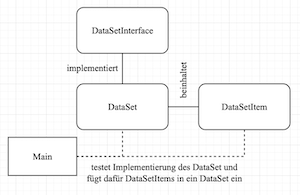
\includegraphics[width=\textwidth]{C:/Users/nourk/OneDrive/Desktop/Git-2024-25/diagram/classes_files.pdf}
\caption{Darstellung der Beziehungen zwischen den Klassen DataSetInterface, DataSet und DataSetItem}
\label{fig:diagram}
\end{figure}

% Abschnitt 3: Abgabe
\section{Abgabe}
Implementieren Sie die Klasse \texttt{DataSet} in der Datei \texttt{implementation.py} zur Lösung der oben beschriebenen Aufgabe.

Sie können auch lokal auf Ihrem Computer arbeiten. Alle drei benötigten Dateien sind im Moodle zum Download verfügbar.

Das VPL verwendet den gleichen Code, wobei \texttt{main.py} zusätzliche Testfälle und Prüfungen enthält.

\hrule
\vspace{1cm}
\footnotesize{Dateien befinden sich im Ordner \texttt{/code/} dieses Git-Repositories.}

\end{document}